\documentclass{article}

\usepackage[utf8]{inputenc}
\usepackage{geometry}
\usepackage{graphicx}
\usepackage[table]{xcolor}% http://ctan.org/pkg/xcolor
\usepackage{algorithm}% http://ctan.org/pkg/algorithms
\usepackage{algpseudocode}% http://ctan.org/pkg/algorithmicx

\usepackage{hyperref}
\usepackage{amsmath}


\usepackage{float}

\delimitershortfall-1sp
\newcommand\abs[1]{\left|#1\right|}


\title{Algoritmo: Subsecuencia Común Más Larga}
\author{Sergio García Prado}


\begin{document}

\begin{titlepage}
	\centering
	{\scshape\LARGE Universidad de Valladolid \par}
	\vspace{1cm}
	{\scshape\Large Programación Dinámica\par}
	\vspace{1.5cm}
	{\huge\bfseries Subsecuencia Común Más Larga\par}
	\vspace{2cm}
	{\Large\itshape Sergio García Prado\par}

	\vfill
	Seguimiento del trabajo en: \par
	\href{https://github.com/garciparedes/Longest-Common-Subsequence}{https://github.com/garciparedes/Longest-Common-Subsequence}

	\vfill


% Bottom of the page
	{\large \today\par}
\end{titlepage}

\section{Introducción}

	\subsection{Definición del problema}

		\paragraph{}
		El problema analizado que se pretende resolver consiste en lo siguiente:

		\paragraph{}
		Primeramente describiremos lo que es una secuencia para después explicar el significado de subsecuencia, ya que es una de las ideas fundamentales que habrá que tener claro para entender los requisitos del problema, que no debemos confundir con el concepto de  subcadena.

		\paragraph{Secuencia:}
		Es una colección ordenada de elementos en la cual la repetición está permitida.
		\newline{}
		Ejemplo: {A, B, C, A, E, F}

		\paragraph{Subsecuencia:}
		Es una secuencia que se obtiene a partir de otra secuencia de igual o mayor longitud mediante la supresión de algunos elementos manteniendo el orden de los elementos restantes. Por ejemplo, la secuencia A, C, A es una subsecuencia de A, B, C, A, E, F.
		\newline
		No debe confundirse con el término subcadena, que además impone la restricción de que los elementos han de ser contiguos. Un ejemplo de subcadena es  C, A, E.

		\paragraph{}
		Ahora que ya tenemos clara la definición de subsecuencia modelizaremos el problema a resolver:
		
		\paragraph{}
		\textbf{Dadas dos secuencias de longitud arbitraria, nuestro objetivo es encontrar la subsecuencia común de mayor longitud entre ambas.}

	\subsection{Aplicaciones}
	
		\paragraph{}
		Este algoritmo tiene una gran cantidad de aplicaciones. Uno de los sectores donde su uso está más extendido es en el de la informática: se usa en software de control de versiones como \textbf{git} o en el comando \textbf{diff} de linux, que muestra las diferencias entre ficheros. También se utiliza en el sector de la bioinformática (Aplicación de la tecnología de computadores a la gestión y análisis de datos biológicos.) para \textbf{secuenciación de ADN}.

\section{Programación Dinámica}

	\subsection{Definición}
	
		\paragraph{}
		La programación dinámica es un patrón de diseño de algoritmos basado en la división del problema base en subproblemas de menor tamaño y complejidad que solo se resolverán una única vez, ya que se almacenará la solución de cada uno de ellos para luego reutilizarlo en el caso de que fuera necesario. Al proceso de almacenar las soluciones de los subproblemas se lo denomina \textbf{memoization}. Para que un problema pueda ser resuelto mediante programación dinámica este tiene que cumplir dos propiedades: solapamiento de los subproblemas y subestructura óptima.

	\subsection{Solapamiento de Problemas}
		\paragraph{}
		Se dice que un problema tiene esta propiedad si este se puede subdividir en problemas de menor tamaño cuyos resultados se pueden reutilizar para resolver sucesivos subproblemas. El ejemplo más claro de esta propiedad es la Sucesión de Fibonacci, que se define como:

		\[
   		 F(n)=
			\begin{cases}
    				n					& \text{if } n\leq 1\\
    				F( n - 1) + F(n - 2)		& \text{otherwise}
			\end{cases}
		\]

		\paragraph{}
		Gráficamente esto se puede representar como un arbol binario, en el cual, para calcular un nodo, tenemos que recurrir a los resultados de sus dos hijos, y así sucesivamente hasta llegar a tener como hijos$F(0), F(1)$, que son nuestros casos base:

		\begin{figure}[H]
				\centering
				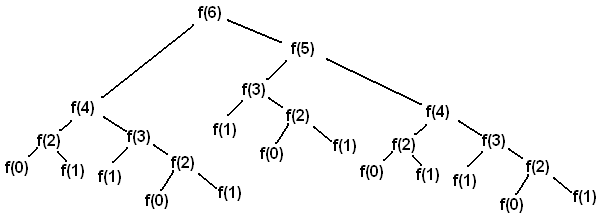
\includegraphics[width=120mm]{../res/fibonacci-sequence.png}
				\caption{Sucesión de Fibonacci \label{example_border}}
		\end{figure}

	\subsection{Subestructura Óptima}
	
		\paragraph{}
		La segunda propiedad que debe cumplir el problema es la de subestructura óptima, que consiste en lo siguiente: La solución al problema contiene (o depende) de las soluciones óptimas a sus subproblemas. Esta es una propiedad que la programación dinámica comparte con los algoritmos voraces.

\section{Solución}

	\subsection{Enfoques Disponibles}
	
		\paragraph{}
		Para resolver el problema de encontrar la subsecuencia común más larga entre $N[n_{1}...n_{n}]$ secuencias existen distintos enfoques:

		\paragraph{}
		 Primeramente podríamos pensar en un enfoque por fuerza bruta, es decir, comparando todas las subsecuencias posibles. Esto tendría un crecimiento asintótico de $O(2^{n_{1}}\sum_{i = 2}^{N}n_{i})$ que corresponde al coste de obtener todas las subsecuencias de la primera secuencia $O(2^{n_{1}})$ y compararlo con todas las demás  (sumatorio de todas las restantes), es decir, de compararlas todas con todas.

		\paragraph{}
		 Otra solución es utilizar un enfoque dinámico, ya que como demostraremos posteriormente, nuestro problema posee las propiedades necesarias para ser resuelto de esta manera. Con este enfoque obtenemos un crecimiento asintótico de  $O(N\prod_{i = 1}^{N}n_{i})$ que corresponde al coste de generar la matriz que almacena las longitudes de subsecuencias comunes (memoization).

		\paragraph{}
		Nótese que para valores muy grandes de N el problema se transforma en uno de tipo \textbf{NP-hard}, es decir, problemas de decisión que son como mínimo tan difíciles como un problema de NP.

	\subsection{Enfoque dinámico}

		\paragraph{}
		Veamos como encontrar la subsecuencia común más larga se puede resolver por programación dinámica. Abordaremos el problema para dos secuencias, pero este es extrapolable a cualquier número de secuencias fácilmente incrementando el tamaño de la entrada de nuestro algoritmo.

		\subsubsection{Notación}

			\paragraph{}
			Denominaremos a las dos secuencias $X[0...m-1]$ e $Y[0...n-1]$ cuya longitud será m y n respectivamente. 		
			\newline{}
			A modo de ejemplo supondremos $X = abcde, Y = aert$ por lo que $m = 5, n = 4$.
			
			\paragraph{}
			También que tenemos una matriz de L[0...m-1][0...n-1] de tamaño m x n, la cual  utilizaremos para almacenar los resultados de cada subproblema
			
			\paragraph{}
			Sea $S$ una secuencia, $l$ su longitud  e $i \in (1, l)$, la secuencia $S_{i}$ es la correspondiente a los $i$ primeros elementos. 
			\newline{}
			Ejemplo: $X_{1} = a$, $X_{3} = abc$ y $X_{5} = abcde = X$
			
		\subsubsection{Subestructura óptima}

			\paragraph{}
			En el caso de que X[m-1] sea igual a Y[n-1] (las últimas posiciones de cada secuencia), rellenaremos la matriz L con el valor de las secuencias sin esos últimos elementos + 1 (el elemento común encontrado):
			\[
			L(X[0..m-1], Y[0..n-1]) = 1 + L(X[0..m-2], Y[0..n-2])
			\]
			\newline{}
			Ejemplo:
			\[
			L(abcde, aert) = 1 + L(abcd, aer)
			\]

			\paragraph{}
			Por contra, si los dos últimos elementos no fueran iguales, es decir, si X[m-1] fuese distinto de Y[n-1] tendríamos que obtener el máximo de eliminar el último carácter de la primera secuencia y de la segunda, es decir:
			\[
			L(X[0..m-1], Y[0..n-1]) = max(L(X[0..m-2], Y[0..n-1]), L(X[0..m-1], Y[0..n-2])
			\]
			\newline{}
			Ejemplo:
			\[
			L(abcd, aer) = max( L(abc, aer), L(abcd, ae) )
			\]

			\paragraph{}
			La formulación completa del problema es la siguiente:
			\[
   			 LCS( X_{i}, Y_{j} ) =
				\begin{cases}
				    	0									& \text{if } i = 0 \vee	 j = 0\\
    					LCS( X_{i-1}, Y_{j-1}) + 1					& \text{if } x_{i} = y_{j}\\
    					max(LCS( X_{i}, Y_{j-1}), LCS( X_{i-1}, Y_{j}))	& \text{if } x_{i} \not = y_{j}
				\end{cases}
			\]

			\paragraph{}
			Para rellenar la matriz L aplicaremos la función $LCS( X_{i}, Y_{j} )$ a cada una de las entradas $L_{ij}$.

		\subsubsection{Solapamiento de problemas}

			\paragraph{}
			Como se puede apreciar, el resultado  de cada subproblema se reutiliza para obtener el de los de nivel superior. Por tanto podemos almacenar el resultado para calcularlo una única vez al igual que en el caso de la Sucesión de Fibonacci..

		\subsubsection{Obtención de los resultados}
		
			\paragraph{}
			Para obtener la longitud de la subsecuencia común más larga tan solo tendremos que obtener el valor de $L_{mn}$. Este valor se encuentra en esa posición dado que es la última entrada de la matriz que se rellena, es decir, el corresponde a las secuencias completas.

			\paragraph{}
			Para obtener la subsecuencia común más larga el proceso es algo más complicado. A grandes rasgos consiste en comenzar en la entrada $L_{mn}$ e ir decrementando los valores de $i$ y $j$ añadiendo a la secuencia el elemento correspondiente a dicha posición en el caso de que $ X_{i} = Y_{j}$ o en caso contrario decrementar $i$ o $j$ según sea mayor $X_{i}$ o  $Y_{j}$ hasta que $i = 0$ o $j = 0$. La secuencia resultante será la subsecuencia común más larga.

			\paragraph{}
			Este algoritmo se puede adaptar fácilmente para encontrar todas las subsecuencias comunes más largas en caso de que esta no fuera única simplemente recorriendo todos los caminos posibles (ya que este puede no ser único) que cumplan las condiciones anteriormente descritas.

		\subsubsection{Ejemplo de ejecución}

			\paragraph{}
			Sean $X = abcde, Y = aert $ por lo que $m = 5, n = 4$.

			\paragraph{}
			Lo primero que haremos es aplicar el algoritmo para generar la matriz $L$.
			\newline{Nota:}
			Para mejorar la eficiencia del algoritmo aumentamos en 1 el tamaño de la matriz, es decir, $L[0...m][0...n]$ para añadir 0 en las entradas $L_{ij}$ tales que $i = 0$ o $j = 0$, lo que reduce el número de comprobaciones respecto de los límites de la lista.

			\begin{center}
	    		\(
	  			\begin{tabular}{ | c | c | c | c | c | c | c | }
	    				\hline
					   & $\emptyset$ & a & b  & c  & d & e \\ \hline
					$\emptyset$ &   &   &    &    &   &    \\ \hline
					a &   &   &    &    &    &    \\ \hline
					e &   &   &    &    &    &   \\ \hline
					r &   &   &    &    &    &   \\ \hline
					t &   &   &    &    &   &    \\
					\hline
				\end{tabular}
			    \)
	    		\hspace{.1in}
	    		\(
	  			\begin{tabular}{ | c | c | c | c | c | c | c | }
	    				\hline
					   & $\emptyset$ & a & b  & c  & d & e \\ \hline
					$\emptyset$ & 0 & 0 & 0  & 0  & 0 & 0  \\ \hline
					a & 0 &   &    &    &    &    \\ \hline
					e & 0 &   &    &    &    &   \\ \hline
					r & 0 &   &    &    &    &   \\ \hline
					t & 0  &   &    &    &   &    \\
					\hline
				\end{tabular}
			    \)
	    		\hspace{.1in}
	    		\(
	  			\begin{tabular}{ | c | c | c | c | c | c | c | }
	    				\hline
					   & $\emptyset$ & a & b  & c  & d & e \\ \hline
					$\emptyset$ & 0 & 0 & 0  & 0  & 0 & 0  \\ \hline
					a & 0 & 1 &    &    &    &    \\ \hline
					e & 0 &   &    &    &    &   \\ \hline
					r & 0 &   &    &    &    &   \\ \hline
					t & 0  &   &    &    &   &    \\
					\hline
				\end{tabular}
			    \)
	    		\hspace{.1in}
	    		\(
				\begin{tabular}{ | c | c | c | c | c | c | c | }
	    				\hline
					   & $\emptyset$ & a & b  & c  & d & e \\ \hline
					$\emptyset$ & 0 & 0 & 0  & 0  & 0 & 0  \\ \hline
					a & 0 & 1 & 1   &    &    &    \\ \hline
					e & 0 &   &    &    &    &   \\ \hline
					r & 0 &   &    &    &    &   \\ \hline
					t & 0  &   &    &    &   &    \\
					\hline
				\end{tabular}
			    \)
	    		\hspace{.1in}
	    		\(
				\begin{tabular}{ | c | c | c | c | c | c | c | }
	    				\hline
					   & $\emptyset$ & a & b  & c  & d & e \\ \hline
					$\emptyset$ & 0 & 0 & 0  & 0  & 0 & 0  \\ \hline
					a & 0 & 1 & 1 & 1 & 1 & 1 \\ \hline
					e & 0 & 1 &    &    &    &   \\ \hline
					r & 0 &   &    &    &    &   \\ \hline
					t & 0  &   &    &    &   &    \\
					\hline
				\end{tabular}
			    \)
	    		\hspace{.1in}
	    		\(
				\begin{tabular}{ | c | c | c | c | c | c | c | }
	    				\hline
					   & $\emptyset$ & a & b  & c  & d & e \\ \hline
					$\emptyset$ & 0 & 0 & 0  & 0  & 0 & 0  \\ \hline
					a & 0 & 1 & 1 & 1 & 1 & 1 \\ \hline
					e & 0 & 1 & 1 & 1 & 1 & 2 \\ \hline
					r & 0 &   &    &    &    &   \\ \hline
					t & 0  &   &    &    &   &    \\
					\hline
				\end{tabular}
			    \)
	    		\hspace{.1in}
	    		\(
				\begin{tabular}{ | c | c | c | c | c | c | c | }
	    				\hline
					   & $\emptyset$ & a & b  & c  & d & e \\ \hline
					$\emptyset$ & 0 & 0 & 0  & 0  & 0 & 0  \\ \hline
					a & 0 & 1 & 1 & 1 & 1 & 1 \\ \hline
					e & 0 & 1 & 1 & 1 & 1 & 2 \\ \hline
					r & 0 & 1 & 1 & 1 & 1 & 2 \\ \hline
					t & 0  &   &    &    &   &    \\
					\hline
				\end{tabular}
			    \)
	    		\hspace{.1in}
	    		\(
				\begin{tabular}{ | c | c | c | c | c | c | c | }
	    				\hline
					   & $\emptyset$ & a & b  & c  & d & e \\ \hline
					$\emptyset$ & 0 & 0 & 0  & 0  & 0 & 0  \\ \hline
					a & 0 & 1 & 1 & 1 & 1 & 1 \\ \hline
					e & 0 & 1 & 1 & 1 & 1 & 2 \\ \hline
					r & 0 & 1 & 1 & 1 & 1 & 2 \\ \hline
					t & 0  & 1 & 1 & 1 & 1 & 2 \\
					\hline
				\end{tabular}
		    	\)
			\end{center}

			\paragraph{}
			Una vez  rellenada la matriz ya conocemos la longitud de la subsecuencia común más larga, que, como dijimos antes se aloja en $L_{mn}$, es decir, $L_{65}$ ya que en nuestro caso la matriz es más grande (sino sería $L_{54}$).

			\paragraph{}
			Para obtener la subsecuencia común más larga utilizaremos el algoritmo expuesto anteriormente:

			\begin{center}
	    		\(
	  			\begin{tabular}{ | c | c | c | c | c | c | c | }
	    				\hline
					   & $\emptyset$ & a & b  & c  & d & e \\ \hline
					$\emptyset$ & 0 & 0 & 0  & 0  & 0 & 0  \\ \hline
					a & 0 & 1 & 1 & 1 & 1 & 1 \\ \hline
					e & 0 & 1 & 1 & 1 & 1 & 2 \\ \hline
					r & 0 & 1 & 1 & 1 & 1 & 2 \\ \hline
					t & 0  & 1 & 1 & 1 & 1 & \cellcolor{blue!25}2 \\
					\hline
				\end{tabular}
			    \)
	    		\hspace{.1in}
	    		\(
				\begin{tabular}{ | c | c | c | c | c | c | c | }
	    				\hline
					   & $\emptyset$ & a & b  & c  & d & e \\ \hline
					$\emptyset$ & 0 & 0 & 0  & 0  & 0 & 0  \\ \hline
					a & 0 & 1 & 1 & 1 & 1 & 1 \\ \hline
					e & 0 & 1 & 1 & 1 & 1 & 2 \\ \hline
					r & 0 & 1 & 1 & 1 & 1 & \cellcolor{blue!25}2 \\ \hline
					t & 0  & 1 & 1 & 1 & 1 & \cellcolor{blue!25}2 \\
					\hline
				\end{tabular}
			    \)
	    		\hspace{.1in}
	    		\(
				\begin{tabular}{ | c | c | c | c | c | c | c | }
	    				\hline
					   & $\emptyset$ & a & b  & c  & d & e \\ \hline
					$\emptyset$ & 0 & 0 & 0  & 0  & 0 & 0  \\ \hline
					a & 0 & 1 & 1 & 1 & 1 & 1 \\ \hline
					e & 0 & 1 & 1 & 1 & 1 & \cellcolor{blue!50}2 \\ \hline
					r & 0 & 1 & 1 & 1 & 1 & \cellcolor{blue!25}2 \\ \hline
					t & 0  & 1 & 1 & 1 & 1 & \cellcolor{blue!25}2 \\
					\hline
				\end{tabular}
			    \)
	    		\hspace{.1in}
	    		\(
				\begin{tabular}{ | c | c | c | c | c | c | c | }
	    				\hline
					   & $\emptyset$ & a & b  & c  & d & e \\ \hline
					$\emptyset$ & 0 & 0 & 0  & 0  & 0 & 0  \\ \hline
					a & 0 & 1 & 1 & 1 & \cellcolor{blue!25}1 & 1 \\ \hline
					e & 0 & 1 & 1 & 1 & 1 & \cellcolor{blue!50}2 \\ \hline
					r & 0 & 1 & 1 & 1 & 1 & \cellcolor{blue!25}2 \\ \hline
					t & 0  & 1 & 1 & 1 & 1 & \cellcolor{blue!25}2 \\
					\hline
				\end{tabular}
			    \)
	    		\hspace{.1in}
	    		\(
				\begin{tabular}{ | c | c | c | c | c | c | c | }
	    				\hline
					   & $\emptyset$ & a & b  & c  & d & e \\ \hline
					$\emptyset$ & 0 & 0 & 0  & 0  & 0 & 0  \\ \hline
					a & 0 & \cellcolor{blue!50}1 & \cellcolor{blue!25}1 & \cellcolor{blue!25}1 & \cellcolor{blue!25}1 & 1 \\ \hline
					e & 0 & 1 & 1 & 1 & 1 & \cellcolor{blue!50}2 \\ \hline
					r & 0 & 1 & 1 & 1 & 1 & \cellcolor{blue!25}2 \\ \hline
					t & 0  & 1 & 1 & 1 & 1 & \cellcolor{blue!25}2 \\
					\hline
				\end{tabular}
			    \)
	    		\hspace{.1in}
	    		\(
				\begin{tabular}{ | c | c | c | c | c | c | c | }
	    				\hline
					   & $\emptyset$ & a & b  & c  & d & e \\ \hline
					$\emptyset$ & \cellcolor{blue!25}0 & 0 & 0  & 0  & 0 & 0  \\ \hline
					a & 0 & \cellcolor{blue!50}1 & \cellcolor{blue!25}1 & \cellcolor{blue!25}1 & \cellcolor{blue!25}1 & 1 \\ \hline
					e & 0 & 1 & 1 & 1 & 1 & \cellcolor{blue!50}2 \\ \hline
					r & 0 & 1 & 1 & 1 & 1 & \cellcolor{blue!25}2 \\ \hline
					t & 0  & 1 & 1 & 1 & 1 & \cellcolor{blue!25}2 \\
					\hline
				\end{tabular}
		    	\)
			\end{center}

			\paragraph{}
			Los resultados de la ejecución para las secuencias $abcde$ y $aert$ son los siguientes; $LCS = ae$ y su longitud 2.
			
	\subsection{PseudoCódigo}

		\begin{algorithm}[H]

			\caption{lcs}

			\label{lcs}

			\begin{algorithmic}[1] % The number tells where the line numbering should start

			\Function{lcs}{$X, Y, m, n) $}
				\State $X:$ secuencia de m elementos [0...m-1]
				\State $Y:$ secuencia de n elementos [0...n-1]
				\State $m:$ longitud de X
				\State $n:$ longitud de Y
				\State

				\State $L \gets array[0...m][0...n]$
				\Comment{O(1)}
				\State


				\For{$i\gets 0, i < m+1, i++$}
				\Comment{$O(m*n)$}

					\For{$j\gets 0, i < n+1, j++$}
					\Comment{O(n)}

						\If{$i = 0 \vee j = 0$}
						\Comment{O(1)}

							\State $L[i][j]\gets 0$
							\Comment{O(1)}

						\ElsIf{$X[i-1] =Y[j-1]$}
						\Comment{O(1)}

 							\State $L[i][j]\gets L[i-1][j-1] + 1$
							\Comment{O(1)}

						\Else

 							\State $L[i][j]\gets max(L[i-1][j], L[i][j-1])$
							\Comment{O(1)}

						\EndIf

					\EndFor

				\EndFor

				\State

				\State $index \gets L[m][n]$
				\Comment{O(1)}
										
				\State $LCS \gets array[0...index-1]$
				\Comment{O(1)}
				\State

				\State $i \gets m$
				\Comment{O(1)}
				
				\State $j \gets n$
				\Comment{O(1)}
		
				\While{$i > 0 \wedge j > 0$}
						\Comment{$O(\frac{n+m}{2})$}
				
					\If{$X[i-1] = Y[j-1]$}
					\Comment{O(1)}
   				
						\State $LCS[index-1]\gets X[i-1]$
						\Comment{O(1)}
				
						\State $index\gets index - 1$
						\Comment{O(1)}
 				
						\State $j\gets j - 1$
						\Comment{O(1)}
 				
						\State $j\gets j - 1$
						\Comment{O(1)}

					\ElsIf{$L[i-1][j] > L[i][j-1]$}
					\Comment{O(1)}
 				
						\State $i\gets i - 1$
						\Comment{O(1)}
				
					\Else
 				
						\State $j\gets j - 1$
						\Comment{O(1)}
				
					\EndIf
				
				\EndWhile
				
				\State

				\State \textbf{return} $LCS$
				\Comment{O(1)}

			\EndFunction
			
			\end{algorithmic}

		\end{algorithm}

	\subsection{Análisis asintótico}
		\paragraph{}
		Como vemos, el orden de crecimiento de la función depende de la longitud de las secuencias de entrada, es decir, del coste de recorrer la matriz $L$
		\[
		T(n) = O(lenX*lenY) + O(\frac{lenX+lenY}{2}) = O(lenX*lenY)
		\]
		Con esto llegamos a la conclusión de que este algoritmo tienen un coste de $O(n^2)$
		
	\section{Referencia Bibliográfica}

		\begin{itemize}
			\item \url{https://en.wikipedia.org/wiki/Sequence}
			\item \url{https://en.wikipedia.org/wiki/Subsequence}
			\item \url{https://en.wikipedia.org/wiki/Bioinformatics}
			\item \url{https://en.wikipedia.org/wiki/Dynamic_programming}
			\item \url{https://www.cs.berkeley.edu/~vazirani/algorithms/chap6.pdf}
			\item \url{https://en.wikibooks.org/wiki/Algorithms/Dynamic_Programming}
			\item \url{http://faculty.ksu.edu.sa/Alsalih/CSC%20529/5.2_DynamicProgramming.pdf}
			\item \url{http://www.geeksforgeeks.org/dynamic-programming-set-4-longest-common-subsequence/}

		\end{itemize}

\end{document}
